% =====================================================================
%  Chapter 10 — The Frictions: Costs, Spreads, and Taxes
% =====================================================================

\chapter{The Frictions: Costs, Spreads, and Taxes}
\label{ch:frictions}

Every edge in this book is quoted against a frictionless benchmark, and
every frictionless benchmark is a fiction. This chapter fixes the
frictions for the reader's particular position --- one investor, liquid
exchange-traded funds, a taxable account and a tax-exempt account --- and
quantifies each.

\section{Costs: what a single investor actually pays}

The friction has three parts, and for this reader they are small but not
zero.

\textbf{The bid--ask spread.} Every trade crosses the spread\idx{Spread}, and the
book charges half a spread per one-way trade, which is the correct
first-order charge: you buy at the offer and sell at the bid, so a round
trip costs one full spread. For a liquid broad-market fund the spread is
typically a basis point or two; for a sector or factor fund it can be ten
times that. The book's model charges two basis points on the most liquid
funds and six on the rest, and Chapter 33 reports the sensitivity of the
result to doubling and tripling those numbers.

The spread is the friction the Securities and Exchange Commission
explicitly warns about: in its investor bulletin on exchange-traded funds,
the Commission notes that the bid--ask spread\idx{Bid-ask spread} is a cost to the investor
that is not visible in the expense ratio\idx{Expense ratio}, and that most funds publish
their median spread on their own website. It is the single most common
hidden cost in the retail ETF account.

\textbf{Commissions.} The book's model charges none, because at the
brokerages this reader is likely to use, a small monthly basket of
liquid ETFs trades commission-free. The commissions\idx{Commissions} a reader at a paying
broker pays are the second friction the book's cost model does not
charge. This is a modelling choice and it is favourable to the system; a
reader at a paying broker should add their own per-trade cost. Chapter 33
reports the result under a cost regime
that is ten times the book's assumption.

\textbf{Expense ratios.} These are \emph{not} charged separately, and the
reason is worth stating because getting it wrong is the single most
common double-counting error in backtests.

The book's return series are built from the raw price and the dividend
components, which excludes the effect of the expense ratio; the
\emph{adjusted close} series that Yahoo publishes embeds it. The book
therefore rebuilds returns from price and dividends so that the gross and
taxable simulations share one set of numbers, and then \emph{checks} the
reconstruction against the adjusted close, which returns a mean absolute
discrepancy of about 0.004 per cent a month --- the difference is
attributable to the dividend-bucket convention and is three orders of
magnitude smaller than the quantity being measured.

The expense ratio is therefore already in the price series. Charging it a
second time would double-count the most certain drag in the whole
calculation. The universe's expense ratios are reported in Appendix C, and
they are real: the cheapest funds are around four basis points and the
most expensive around fifty-five.

\section{Structure: why an ETF is the right wrapper, and what it costs}

The choice of vehicle is not neutral, and the tax treatment of the wrapper
is one of the larger structural advantages available to a small investor.

An exchange-traded fund\idx{Exchange-traded fund} that sells securities in kind --- that is, that
delivers the securities themselves to the shareholders who are selling,
rather than selling them for cash and distributing the proceeds --- can
avoid realizing capital gains inside the fund when its shareholders trade.
The consequence is visible in the distribution statistics: in 2025, about
7 per cent of ETFs distributed a capital gain, against about 52 per cent
of mutual funds; over the long run the figures are about 9 per cent against
53 per cent. The split by strategy is similar in direction and larger in
the passive case: passive ETFs at 4 per cent against passive mutual funds
at 41 per cent.

This is a structural advantage of the wrapper that has nothing to do with
the investor's skill or size, and it is one reason the book's universe is
ETFs rather than funds of any other kind. It is also why the book treats
an in-kind redemption as the default and a cash creation as the exception
in its discussion of the mechanism.

The counterweight is that ETF structure does not exempt the investor from
tax. A gain realised in the investor's own account is a taxable event,
whether the underlying holding was an ETF or a mutual fund, and the
wrapper's efficiency shows up in the fund's distribution, not in the
investor's realisation.

\section{Taxes: the rules the engine implements}

The book maintains two accounts in parallel, with identical weight paths:
one taxable, one tax-exempt. The tax engine implements the following.

\textbf{Holding period.} A position held for more than one year is
long-term; one year or less is short-term. Long-term capital gains are
taxed at preferential rates, which for 2025 means a maximum of 15 per cent
for most taxpayers, with 0 per cent and 20 per cent brackets applying in
the ordinary way. Short-term capital gains are taxed as ordinary income.
The distinction is worth several percentage points a year and it is the
single largest reason the book's taxable account lags its tax-exempt
twin.

\textbf{Ordinary dividends and the qualified dividend\idx{Qualified dividend} tax rate.} Dividends
are taxed as ordinary income, with the exception of the qualified dividend
tax rate applied to the portion of a dividend that qualifies. The book
models a 15 per cent long-term rate on qualified dividends and adds the
3.8 per cent net investment income tax for the higher-income taxpayer, who
is the reader this book is written for.

\textbf{The capital-loss offset.} A net capital loss may offset up to
\$3,000 of ordinary income in a year --- \$1,500 for a married filing
separately --- and the unused portion carries forward indefinitely. The
engine implements the offset and the carryforward.

\textbf{The wash-sale rule, in both directions.} This is the rule that
changes the arithmetic most, and it is the one most often implemented
incorrectly. If a loss is realised on a security and the same or a
substantially identical security is purchased within thirty days before or
after the sale, the loss is disallowed. The disallowed loss is added to the
basis of the replacement shares, and the holding period of the replacement
tacks onto the holding period of the original shares.

Two consequences matter for a system. First, the rule operates in both
directions, so a system that buys a security within thirty days of a sale
at a loss has its loss disallowed --- the system cannot simply ignore the
rule when it is buying, only when it is selling. Second, because the basis
and the holding period carry over, the rule changes the timing of the tax
and not only its amount, so a wash sale can turn a short-term gain\idx{Short-term gain} into a
long-term one later. The engine tracks lots, applies the thirty-day window
in both directions, adjusts the basis of the replacement, and tacks the
holding period.

\textbf{Inside a tax-exempt account.} The wash-sale disallowance applies
inside an IRA and a Roth IRA as well. A loss realised in the taxable
account whose replacement purchase occurs inside the IRA is still
disallowed. This matters for a reader running the two accounts in parallel,
which is exactly what the book does, and it is the reason the two accounts
in the book are not simply the same portfolio with different tax rates.

\begin{figure}[!htbp]
\centering
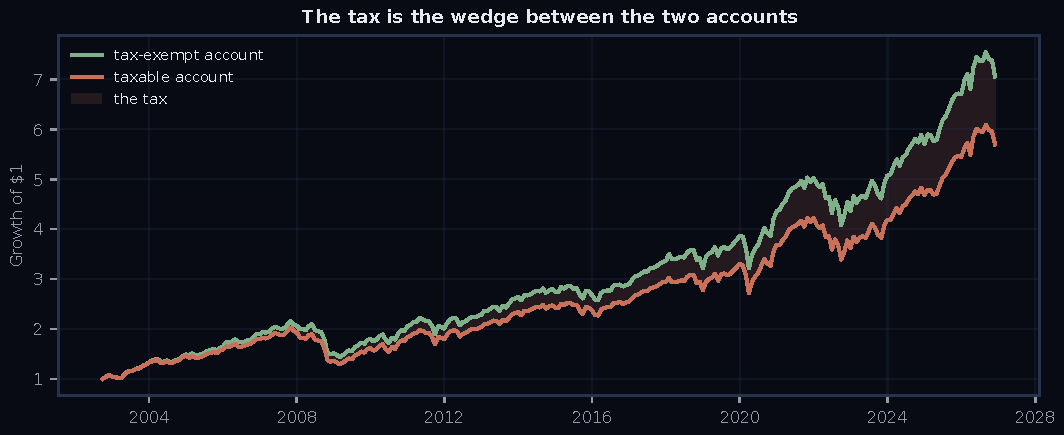
\includegraphics[width=\textwidth]{../figures/fig_tax.pdf}
\caption{The taxable and tax-exempt accounts over the record, and the tax
paid in each year. The gap between the two curves is the price of the tax
code paid by this particular portfolio's trading pattern.}
\label{fig:tax}
\end{figure}

\section{Why taxes belong in the book at all}

The conventional reason is that taxes are a large drag on a high-turnover\idx{Turnover}
strategy and a small one on a low-turnover one. The deeper reason is
different and more useful for this reader.

The tax code is the one part of the market that is not a market. It has no
efficient price, it is set by statute, it changes on a political schedule,
and --- crucially for a system that trades on a signal --- it creates a
\emph{non-linear} cost that depends on the state of the portfolio rather
than on the size of the trade. A spread cost is proportional and
recoverable; a wash sale is a discrete, state-dependent, path-dependent
charge.

A system that ignores the tax code is therefore not simply inaccurate; it
is optimising the wrong objective. And a system that does model it will
make different decisions: it will hold a losing position longer rather
than take the loss, because the replacement purchase inside thirty days
would disallow the loss anyway. That is a real, computable, and slightly
counter-intuitive behaviour, and it is the kind of thing that separates a
system that could be run from one that could only be described.

\begin{keytakeaways}
\item For one investor the friction is the bid--ask spread, the commission,
and the tax code --- not market impact, which is a different problem.
\item Expense ratios are not charged again: the return series already
embeds them, and the reconstruction is checked against the vendor's
adjusted close to a mean discrepancy of about 0.004 per cent a month.
\item The wash-sale rule operates in both directions, adjusts the basis of
the replacement purchase, tacks the holding period, and applies inside an
IRA.
\item Modelling the tax code changes decisions, not just returns: the
system holds a losing position longer rather than crystallising a loss it
could not use.
\end{keytakeaways}
